\chapter{Results and Discussions}
%%%%%%%%%%%%%%%%%%%%%%%%%%%%%%%%%%%%%%%%%%%%%%%%%%%%%%%%%%%%
%%%%%%%%%%%%%%%%%%%%  NEW SECTION   %%%%%%%%%%%%%%%%%%%%%%%%
%%%%%%%%%%%%%%%%%%%%%%%%%%%%%%%%%%%%%%%%%%%%%%%%%%%%%%%%%%%%
\setcounter{equation}{0}

The aim of the system is to provide users with a faster, more reliable and efficient solution for navigating and performing tasks within a banking application that in turn reduces the need for manual repetitive tasks, decreases time loss, and optimizes their productivity.\\

\noindent The main platform used for the development of the system is Python. TensorFlow, a framework in Python, is used to create the OCR model using the implementation of a CNN network model. All the significant sections of code, excluding the front-end interface was purely implemented in Python.\\

\noindent
CNN\_Model\_0 was the initially pitched model plan for the proposed system. It consisted of 7 layers, each layer possessing a small filter size just as in the case of a classical CNN model. CNN\_Model\_1 is an improvement over CNN\_Model\_0, with the addition of a convolutional layer possessing a comparatively bigger filter size. This pushes the advantage of CNN\_Model\_1 over CNN\_Model\_0 by a high margin.\\
 
\begin{table}[ht]
\centering
\caption{Image Size and Channels}
\begin{tabular}{|c|c|c|}
\hline
Image Size & Number of Channels & Channel Name \\
\hline
40x40 & 1 & Grayscale \\
\hline
\end{tabular}
\end{table}

\clearpage

\section{Performance Evaluation}

\begin{figure}[h!]
    \centering
    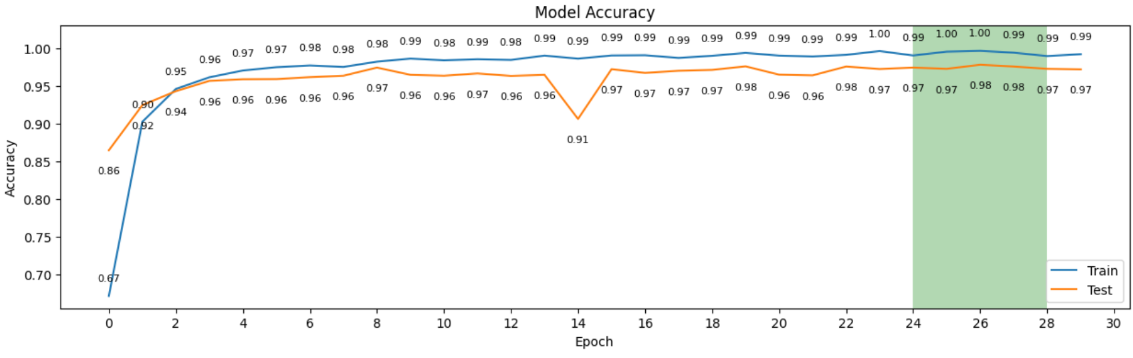
\includegraphics[width=0.9\textwidth]{Images/Perf_Eval/acc_vs_epoch.png}
    \caption{Training accuracy per epoch of CNN Model}
\end{figure}

\noindent CNN\_Model\_0 is improved upon by the addition of a new convolutional layer, which leads to the creation of CNN\_Model\_1. The smallest of changes has an impact on various performance measures related to the CNN model. Though CNN\_Model\_0 outperforms CNN\_Model\_1 in training accuracies, CNN\_Model\_1 gets the upper hand when it comes to validation and testing accuracies. Upon analyzing Figure 4.1, CNN\_Model\_1 has a dip in accuracy during the 14th epoch of training and it can be attributed to a phenomenon called "overfitting".\\

\noindent \textit{Overfitting occurs when the model becomes too specialized in learning the training data, losing its generalization ability to new, unseen data.}\\

\noindent At the 14th epoch, the model might have started to memorize specific patterns in the training set, leading to a decrease in accuracy on the validation data. This memorization can cause the model to perform poorly on examples it has not encountered before, resulting in a temporary drop in accuracy.\\

\noindent As a remedy to this issue, several approaches such as early stopping and regularization can be implemented. But the overall graph shows only a negligible sign of overfitting, indicating effective training and resource utilization. The green shade, representing the best epoch-accuracy range, is prominently located towards the end. This signifies optimal performance without wasting resources.

\clearpage

\noindent
As per the performance, the system is capable of recognizing most of the number written on a paper correctly (Figure 4.2), but still, there are limitations for the model, like the decimal marks (Figure 4.3) or unrecognizable writing styles (Figure 4.4) or due to cut and corrections in the image (Figure 4.5).

\vspace{3mm}

\begin{figure}[h!]
    \centering
    \subfigure{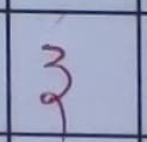
\includegraphics[width=0.2\textwidth,height=0.2\textwidth]{Images/mark_cells/good_mark_cell_1.png}}
    \hspace{10pt}
    \subfigure{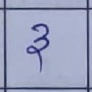
\includegraphics[width=0.2\textwidth,height=0.2\textwidth]{Images/mark_cells/good_mark_cell_2.png}}
    \caption{Cells with mark written correctly}
    
    \vspace{5pt}
    
    \subfigure{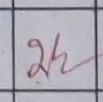
\includegraphics[width=0.2\textwidth,height=0.2\textwidth]{Images/mark_cells/half_mark_cell_1.png}}
    \hspace{10pt}
    \subfigure{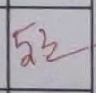
\includegraphics[width=0.2\textwidth,height=0.2\textwidth]{Images/mark_cells/half_mark_cell_2.png}}
    \caption{Cells with half marks (unable to detect)}
    
    \vspace{5pt}
    
    \subfigure{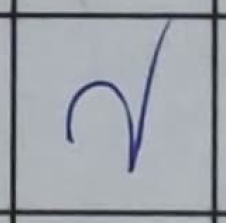
\includegraphics[width=0.2\textwidth,height=0.2\textwidth]{Images/mark_cells/unrecog_mark_cell_1.png}}
    \hspace{10pt}
    \subfigure{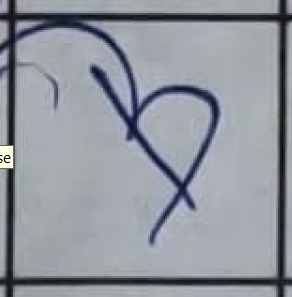
\includegraphics[width=0.2\textwidth,height=0.2\textwidth]{Images/mark_cells/unrecog_mark_cell_2.png}}
    \caption{Cells with hard-to-recognize marks (may give false result)}
    
    \vspace{5pt}
    
    \subfigure{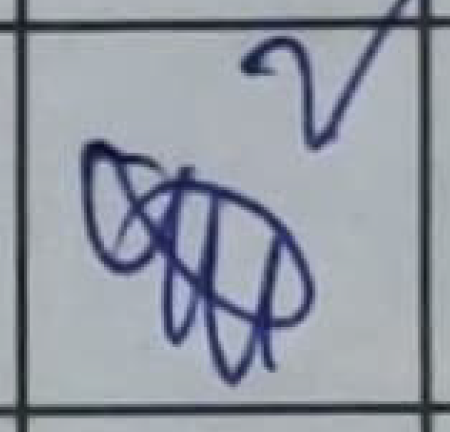
\includegraphics[width=0.2\textwidth,height=0.2\textwidth]{Images/mark_cells/cut_and_correction_mark_cell_1.png}}
    \hspace{10pt}
    \subfigure{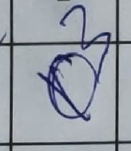
\includegraphics[width=0.2\textwidth,height=0.2\textwidth]{Images/mark_cells/cut_and_correction_mark_cell_2.png}}
    \caption{Cells with cuts and corrections (unable to detect)}
\end{figure}

\clearpage

\section{Comparison with Model Versions}

There have been two versions of the model named CNN\_Model\_0 and CNN\_Model\_1. The two models differ in their purpose and structure.

\subsection{Phases of Model Development}

\textbf{Phase-1: CNN\_Model\_0}

\noindent The CNN\_model\_0 is the 1st model developed that showed par results with the required accuracy, precision, and recall. This model contains 2 convolutional layers, a flattening layer, 3 max-pooling layers, and a dense layer. This model tends to unevenly train all the classes resulting in the high performance of highly trained classes and the low performance of lowly trained classes. Imbalanced learning of classes often leads to a decrease in the classification ability of the model. Operations like image recognition require its effectiveness and are crucial for its practical utility in real-world applications. This problem of uneven learning paved the way for the development of a better model in the next phase.\\

\noindent \textbf{Phase-2: CNN\_Model\_1} 

\noindent This is the fully developed and optimized model that was made by fine-tuning the CNN\_Model\_1 that is used in Marks2csv. It was developed by adding another convolution layer and removing a max-pooling layer. This model thus consists of three Convolutional layers with 16, 32, and 64 filters, each followed by a MaxPooling layer. The output is then flattened and passed through a Dense layer with 64 neurons and ReLU activation. Finally, the output layer has the number of classes with softmax activation for classification. This solved the problem by making all the classes evenly learn to its training data.

\vspace{3mm}

\begin{table}[h]
    \centering
    \begin{tabular}{|c|c|c|c|c|}
    \hline
    Model Name & Epochs & Learning Rate & Layers Count & Features of Layers \\
    \hline
    CNN\_Model\_0 & 30 & 0.001 & 7 & Smaller Filter Size.\\
    \hline
    CNN\_Model\_1 & 30 & 0.001 & 8 & New Conv2D Layer\\
     & & & & And Bigger Filter Sizes.\\
    \hline
    \end{tabular}
    \caption{Comparison Of Two CNN OCR Models}
\end{table}  

\clearpage

\subsection{Comparision of CNN\_Model\_0 and CNN\_Model\_1}

\noindent The models have achieved a testing accuracy of 99\% and 99.2\% for CNN\_Model\_0 and CNN\_Model\_1 respectively. For an in-depth comparison, Table 4.3 is useful as it can be seen that class 3 of CNN\_Model\_0 has a little dip while in the figure of CNN\_Model\_1, the model has learned all classes equally.

\noindent Comparing the confusion matrices (given in Table 4.3), CNN\_Model\_0 showed a slight dip in accuracy for classes 3 and 5, indicating room for improvement. In contrast, CNN\_Model\_1 demonstrated balanced learning across all classes, indicating its ability to classify instances accurately. These insights gives guidance in refining the models for enhanced performance and accuracy.

\noindent The data, given in Table 4.5, compare the performance metrics for the two versions of CNN models. It can be seen that the precision values have not changed with the change in versions. But the recall values have decreased by 0.001 to reach 0.986 in CNN\_ Model\_1. Also, the F1-scores have decreased by 0.011 to reach 0.988 in CNN\_ Model\_1.

\vspace{1 cm}

\begin{table}[h!]
    \centering
    \caption{Accuracy By Class Comparison CNN\_Model\_0 and CNN\_Model\_1}
    \vspace{1.5mm}
    \begin{tabular}{|c|c|}
      \hline
      \textbf{CNN\_Model\_0} & \textbf{CNN\_Model\_1} \\
      \hline
      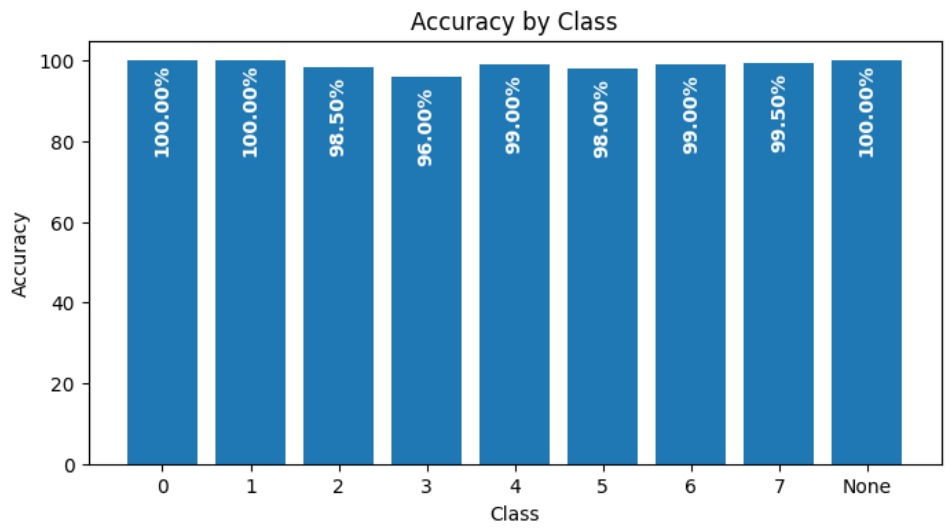
\includegraphics[width=0.5\textwidth]{Images/Perf_Eval/M0_acc_by_cls.png} & 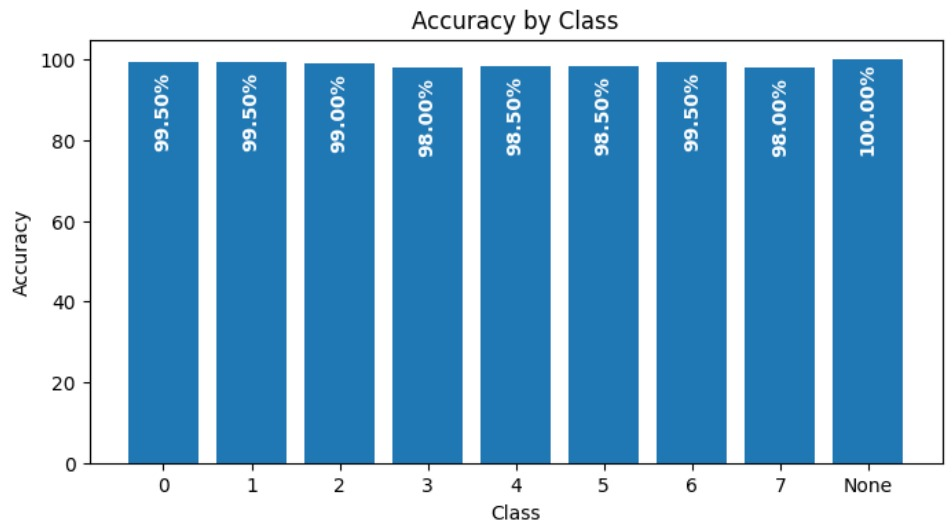
\includegraphics[width=0.5\textwidth]{Images/Perf_Eval/M1_acc_by_cls.png} \\
      \hline
    \end{tabular}
\end{table}

\begin{table}[h!]
    \centering
    \caption{Confusion Matrix Comparison CNN\_Model\_0 and CNN\_Model\_1}
    \vspace{1.5mm}
    \begin{tabular}{|c|c|}
      \hline
      \textbf{CNN\_Model\_0} & \textbf{CNN\_Model\_1} \\
      \hline
      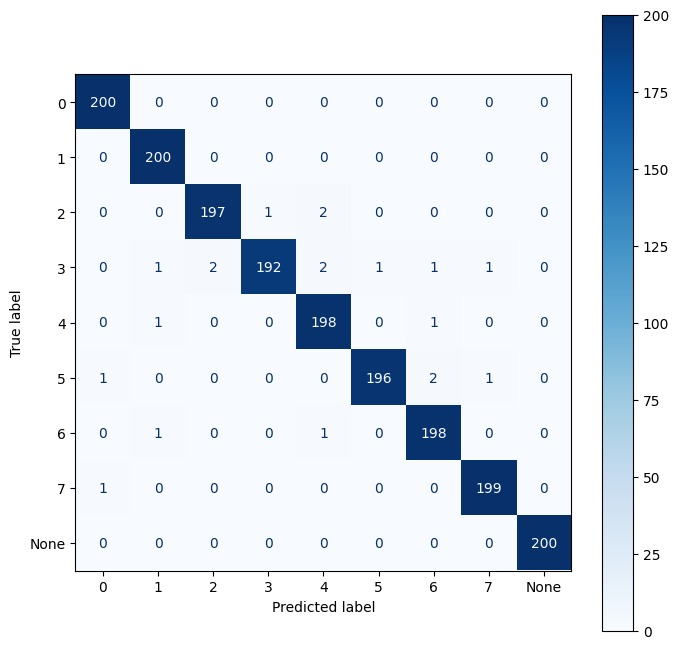
\includegraphics[width=0.5\textwidth]{Images/Perf_Eval/M0_Conf_mat.jpg} & 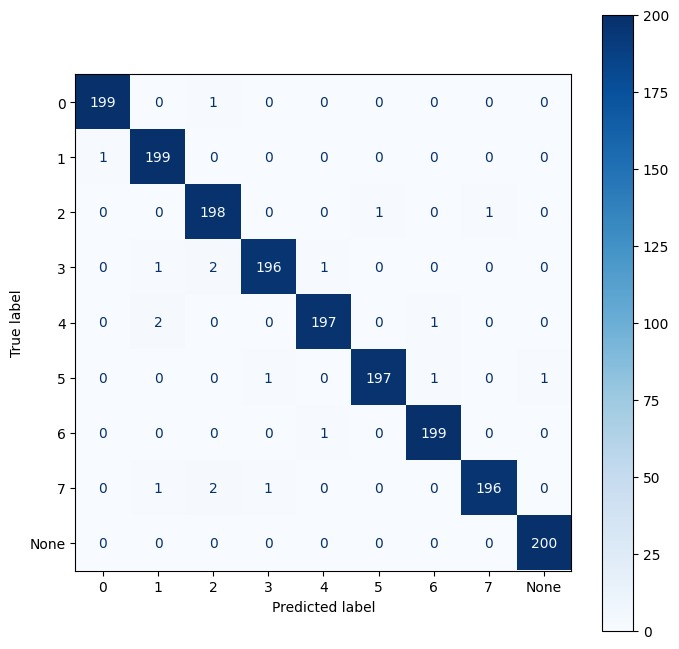
\includegraphics[width=0.5\textwidth]{Images/Perf_Eval/M1_Conf_mat.png} \\
      \hline
    \end{tabular}
\end{table}

\begin{table}[h!]
  \centering
  \caption{Performance metrics comparison for two versions of CNN Models}
  \vspace{1.5mm}
  \begin{tabular}{|c|c|c|c|c|c|c|c|c|c|c|}
  \hline
   & 0 & 1 & 2 & 3 & 4 & 5 & 6 & 7 & \text{None} & \text{Overall} \\ \hline
  \multicolumn{11}{|c|}{\text{CNN\_Model\_0}} \\ \hline
  \text{Precision} & 0.99 & 0.99 & 0.99 & 0.99 & 0.98 & 0.99 & 0.98 & 0.99 & 1 & 0.988 \\ \hline
  \text{Recall} & 1 & 1 & 0.98 & 0.96 & 0.99 & 0.98 & 0.99 & 0.99 & 1 & 0.987 \\ \hline
  \text{F1-Score} & 1 & 0.99 & 0.99 & 0.98 & 0.98 & 0.99 & 0.99 & 0.99 & 1 & 0.999 \\ \hline
  \multicolumn{11}{|c|}{\text{CNN\_Model\_1}} \\ \hline
  \text{Precision} & 0.99 & 0.98 & 0.98 & 0.99 & 0.99 & 0.99 & 0.99 & 0.99 & 1 & 0.988 \\ \hline
  \text{Recall} & 0.99 & 0.99 & 0.99 & 0.98 & 0.98 & 0.98 & 0.99 & 0.98 & 1 & 0.986 \\ \hline
  \text{F1-Score} & 0.99 & 0.99 & 0.98 & 0.98 & 0.99 & 0.99 & 0.99 & 0.99 & 1 & 0.988 \\ \hline
  \end{tabular}
\end{table}

\clearpage

\section{Comparison with State-of-the-Art Methods}

% \vspace{0.3 cm}

The Marks2CSV application utilizes a cutting-edge CNN model developed from scratch, incorporating diverse libraries and modern techniques. This model represents a significant advancement in accuracy, precision, and recall (see Figure 4.7), and can even outperform previous state-of-the-art technologies.

\subsection{Lenet5 vs CNN\_Model\_1}

LeNet-5 is a classic convolutional neural network architecture designed by Yann LeCun et al. in 1998. LeNet-5 was a pioneering CNN architecture that demonstrated the potential of deep learning for image recognition tasks. It laid the foundation for the development of more advanced CNN architectures and significantly contributed to the success of deep learning in various computer vision applications.

\noindent One key advantage of the Marks2CSV application is its exceptional efficiency, providing outputs within seconds. The output is in CSV format, which is both machine-readable and writable, allowing seamless integration with existing data processing workflows. This time-saving capability and data manipulability distinguish Marks2CSV from other tools, making it invaluable for various applications.

\noindent The LeNet5 model, on the other hand, serves the specific purpose of detecting numerical and mathematical operations. While sharing a similar architecture with the CNN model, the divergent outcomes arise from their distinct task focus.

\noindent The Marks2CSV application utilizes the model CNN-Model-1 and is largely comparable to the popular LeNet5. Here is a detailed comparison between the two models:\\

\begin{enumerate}

\item \textbf{Architecture:}

\textbf{CNN\_Model\_1:} 
 It has a simpler architecture with fewer layers and neurons compared to LeNet-5.
\begin{itemize} 
    \item uses 40x40 input images
    \item Convolutional Layers: 3 layers (with 16, 32, and 64 filters)
    \item Max-Pooling Layers: 2 layers
    \item Flatten layer: 1 layer
    \item Hidden Layers: 1 fully connected layer with 64 neurons
    \item Output Layer: 1 fully connected layer with num\_classes neurons (using softmax activation)
    \item uses the ReLU activation function in the fully connected layers

\end{itemize}

\textbf{LeNet5:}  The architecture consists of 7 layers, including 2 convolutional layers and 2 fully connected layers. The LeNet5 model shares a similar architecture with the CNN-Model-1, but it is specifically designed for detecting numerical and mathematical operations.
\begin{itemize}
\item Input Layer: Grayscale images with a shape of 32x32 pixels.

\item Convolutional Layers: 2 layers (with 6 and 16 filters  followed by Tanh activation).

\item Average Pooling Layers: 2 layers of 2x2 pooling with a stride of 2.

\item Fully Connected Layers: 2 layers (120 neurons and 84 neurons with Tanh activation).

\end{itemize}


\item \textbf{Performance:}

\textbf{CNN\_Model\_1:} The CNN-Model-1 demonstrates superior performance compared to previous state-of-the-art technologies. It achieves an accuracy of 0.99, precision of 0.99, and recall of 0.99, indicating its high accuracy in classifying marks from images. It was tested with both ADAM and Stochastic Gradient Descend Optimizers and results show that it is robust and maintained an accuracy of no significant dips in the value. (see Table 4.6)\\

\textbf{LeNet5:} The LeNet5 model achieves a lower accuracy of 0.87, precision of 0.88, and recall of 0.87. While it still performs reasonably well, it falls short compared to CNN-Model-1 in terms of accuracy, precision, and recall. Although it performed as well as CNN-Model-1 in terms of accuracy, Table 4.6 shows a significant dip in precision and recall when using SGD Optimizer.

\clearpage

\item \textbf{Task Focus:}

\textbf{CNN\_Model\_1:}The CNN-Model-1 is designed to handle a broad range of tasks related to marks extraction and processing. It excels in accurately classifying images of whole numbers.\\

\textbf{LeNet5:}The LeNet5 model is specifically tailored for detecting numerical and mathematical operations. It focuses on identifying and recognizing numerical characters, symbols, and mathematical expressions within the images.

\item \textbf{Efficiency:}

\textbf{CNN\_Model\_1:} The Marks2CSV application utilizing CNN-Model-1 offers exceptional efficiency, providing outputs in seconds. This fast delivery of results enables efficient data processing and analysis, enhancing productivity.\\

\textbf{LeNet5:}The efficiency of the LeNet5 model may vary depending on the complexity of the numerical and mathematical operations being detected. However, it is still an effective tool for identifying and extracting specific types of information within the images.

\end{enumerate}

\vspace{1 cm}

\begin{table}[h]
    \centering
    \caption{Tabular comparison of performance metrics (CNN Model and LeNet5)}
    \begin{tabular}{|c|c|c|c|c|c|c|}
    \hline
    \multicolumn{1}{|c|}{\textbf{Optimizer}} & \multicolumn{3}{c|}{\textbf{ADAM Optimizer}} & \multicolumn{3}{c|}{\textbf{SGD Optimizer}} \\ \hline
    \textbf{Model} & \textbf{Accuracy} & \textbf{Precision} & \textbf{Recall} & \textbf{Accuracy} & \textbf{Precision} & \textbf{\textbf{Recall}} \\ \hline
    \textbf{CNN\_Model\_1} & 0.99 & 0.99 & 0.99 & 0.99 & 0.97 & 0.97 \\ \hline
    \textbf{LeNET5} & 0.87 & 0.88 & 0.87 & 0.87 & 0.46 & 0.25 \\ \hline
    \end{tabular}
\end{table}

\clearpage

\noindent Given below is the graphical representation of Table 4.6

\begin{figure}[htbp]
  \centering

  \includegraphics[width=0.45\textwidth]{Images/Results_Discussions/CNN\_Model\_1 ADAM.png}
  \hfill
  \subfigure{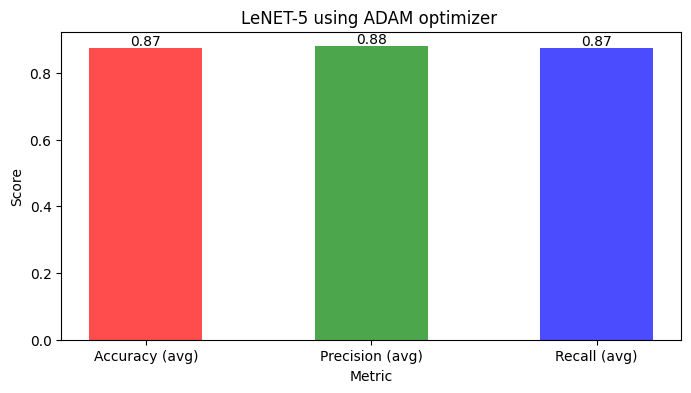
\includegraphics[width=0.45\textwidth]{Images/Results_Discussions/Lanet5 ADAM.png}}
  \caption{Model Comparison: CNN Model 1 vs LeNet5 with ADAM Optimizer}

  \vspace{0.5cm} % Adjust the vertical spacing between the rows of images

  \subfigure{\includegraphics[width=0.45\textwidth]{Images/Results_Discussions/CNN\_Model\_1 SGD.png}}
  \hfill
  \subfigure{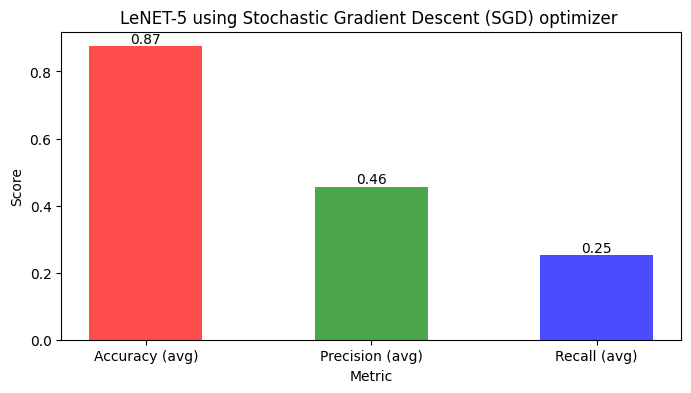
\includegraphics[width=0.45\textwidth]{Images/Results_Discussions/Lanet5 SGD.png}}
  \caption{Model Comparison: CNN Model 1 vs LeNet5 with SGD Optimizer}
  
\end{figure}

\section{Discussion}

In the evaluation of two models, namely CNN-Model-1 and LeNet5, their performance was analyzed using two different optimizers: Adam and SGD. The objective was to assess the impact of optimizer choice on the accuracy of the models.

\noindent When testing CNN-Model-1 with both Adam and SGD optimizers, it was observed that there was no significant change in accuracy. Regardless of the optimizer used, CNN-Model-1 consistently performed well, indicating its robustness and stability. This suggests that the choice of optimizer had minimal influence on the overall accuracy of the model. Thus, CNN-Model-1 demonstrated its superiority by consistently maintaining a high level of accuracy in both optimizer scenarios.

\clearpage

\noindent On the other hand, LeNet5 exhibited a contrasting behavior when tested with Adam and SGD optimizers. While LeNet5 initially showed promising results with the Adam optimizer, a considerable performance drop was observed when switching to the SGD optimizer. This performance degradation indicates that the SGD optimizer was not suitable for the LeNet5 architecture, leading to a significant decrease in accuracy. This discrepancy highlights the sensitivity of LeNet5 to the choice of optimizer and emphasizes the importance of selecting an appropriate optimizer for optimal performance.

\noindent Based on these findings, it is evident that CNN-Model-1 outperformed LeNet5 in both optimizer scenarios. CNN-Model-1 consistently demonstrated higher accuracy and showcased its robustness by maintaining its superior performance regardless of the optimizer choice. These results emphasize the effectiveness and superiority of CNN-Model-1 over LeNet5, positioning it as a more reliable and accurate model for the given task.

\noindent It is worth noting that further analysis and experimentation may be required to determine the underlying factors contributing to the contrasting performances of the two models with different optimizers. Additional investigations into model architecture, dataset characteristics, and hyperparameter tuning could provide valuable insights into the observed performance differences.

% \end{document}